\section{Polygonal Linkages}

Formally, a \textit{polygonal linkage} is an ordered pair $\left(\PP,\HH
\right)$ where $\PP$ is a finite set of polygons and $\HH$ is a finite set of hinges; a 
\textit{hinge} $h\in \HH$ 
corresponds to two points on the boundary of two distinct polygons in $\PP$.  A \emph{realization 
of a polygonal linkage} is an interior-disjoint placement of 
congruent copies of the polygons in $\PP$ such that the copies of a hinge are mapped to the same point (e.g., Figure \ref{fig:linkage-1}).  A \textit{polygonal linkage realization with fixed orientation} allows for any combination of translations and rotated copies of polygons in $\PP$ where every hinge has a cyclic order of  of incident polygons.  Note that oriented polygonal linkage realizations do not allow for reflection transformations.  

These two types of realization types allow one to pose two different types of problems, the realizability problem for polygonal linkages and the realizability problem for polygonal linkages with fixed orientation:
\begin{prob}[Realizibility Problem for Polygonal Linkages]\label{problem:UnorderedPolygonal}
The realizability problem for a polygonal linkage asks whether a given polygonal linkage has 
a realization.
\end{prob}
\begin{figure}[!htbp]
\begin{center}
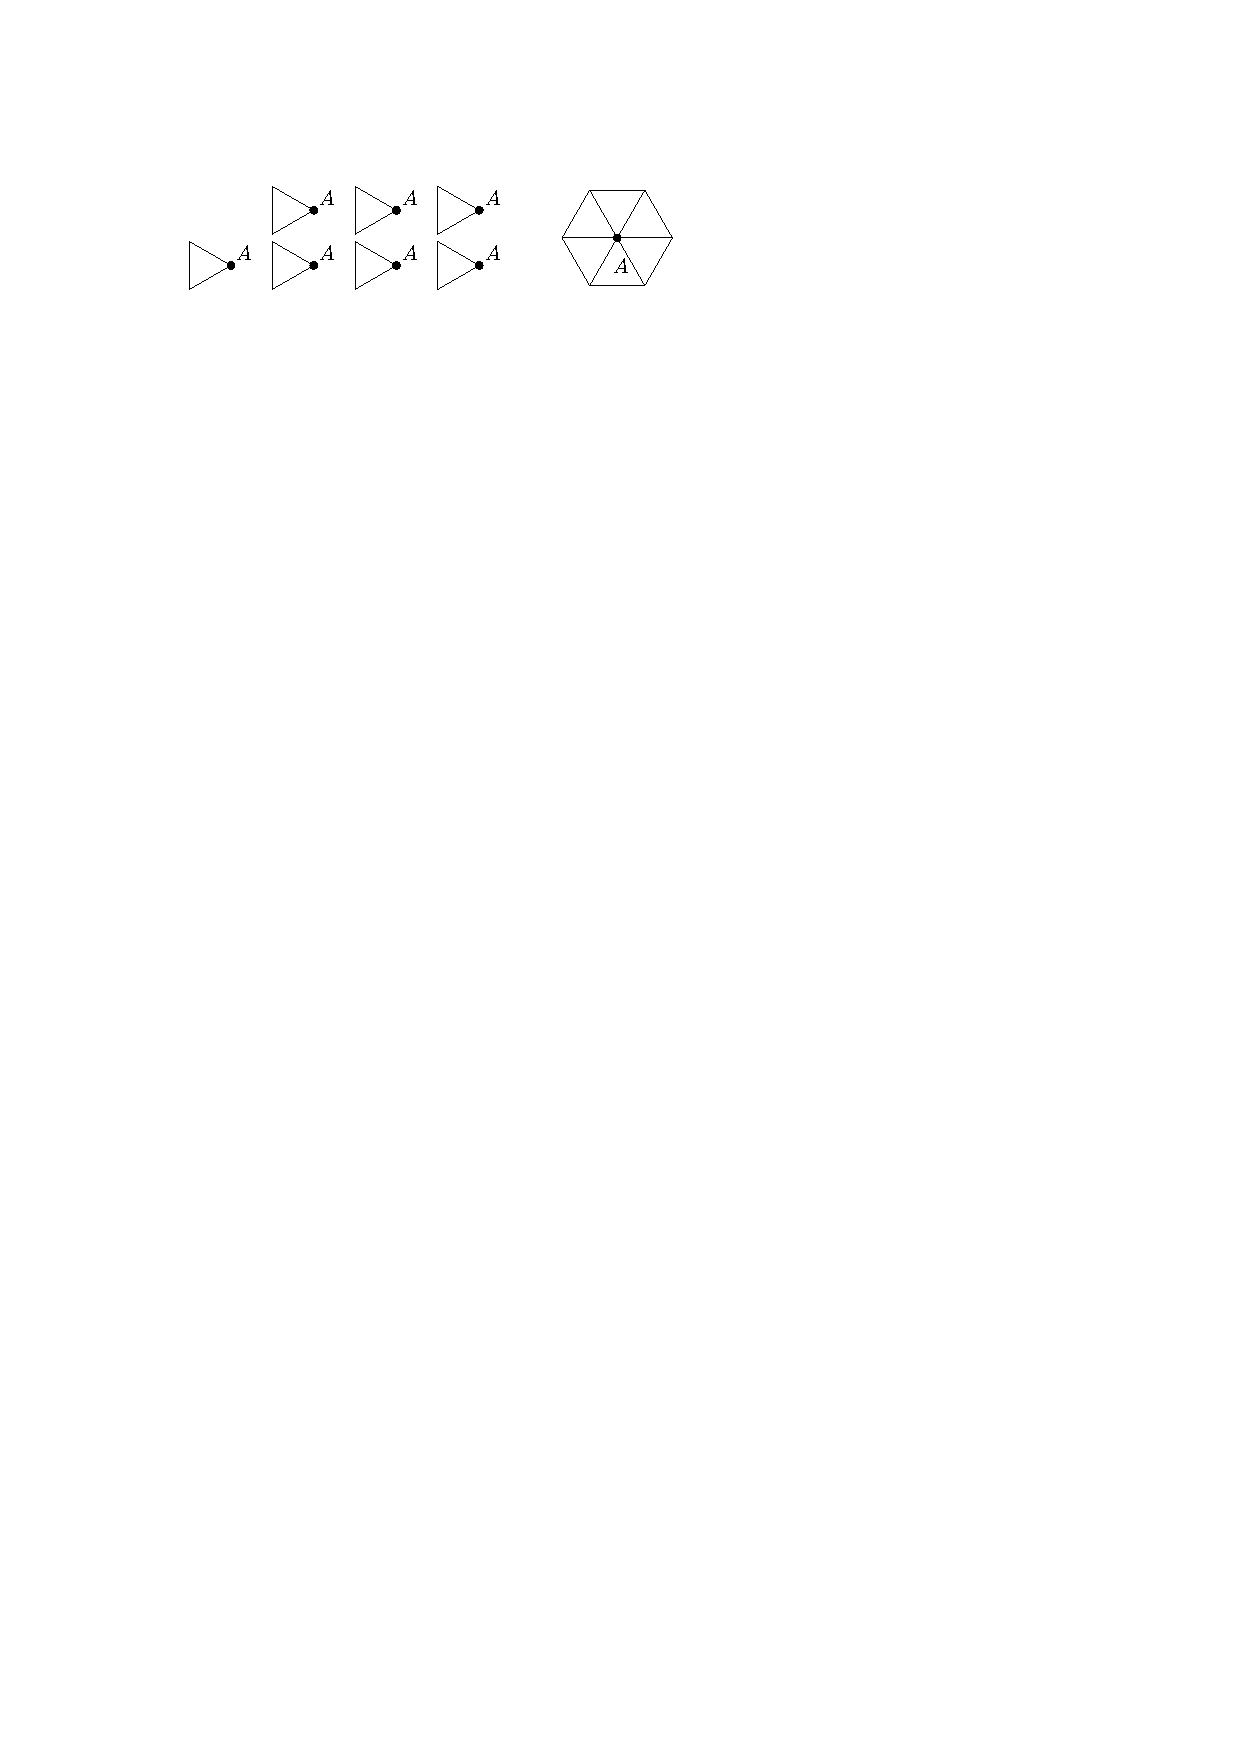
\includegraphics[scale=1]{graphics/Problem1.pdf}
\end{center} 
\caption{Here we have 7 congruent copies of an equilateral triangle with a hinge point of $A$.  The polygonal linkage is not realizable.  The best we can realize is at most 6 congruent copies of an equilateral triangle with the hinge point of $A$ in the plane.}
\label{fig:problem1}
\end{figure}


Figures \ref{fig:problem1} and \ref{fig:collidingHingedPolygons} demonstrates that not all polygonal linkages have a planar realization.  
\begin{figure}[!htbp]\label{fig:collidingHingedPolygons}
\begin{center}
\includegraphics[scale=1]{graphics/collidingHingedPolygons.pdf}
\end{center} 
\caption{This example shows yet another example where two realizations of the same polygonal linkage.  One realization where there is an intersection and another where there isn't an intersection.}
\end{figure}

\begin{figure}[!htbp]
\begin{center}

\includegraphics[scale=1]{graphics/hingeOnThreeDistinctPolygons.pdf}
\end{center} 
\caption{(a) A polygonal linkage with a non-convex polygon and two hinge points corresponding to 
three polygons.  Note that hinge points correspond to two distinct polygons.(b) Illustrating that 
two hinge points can correspond to the same boundary point of a polygon.}
\label{fig:linkage-1}
\end{figure}

\begin{prob}[ Realizibility Problem for Polygonal Linkages with Fixed Orientation]\label{problem:OrderedPolygonal}
The \emph{realizability} problem for a ordered polygonal linkage asks whether a given polygonal 
linkage has a realization with respect to order.
\end{prob}

\begin{figure}[!htbp]\label{fig:orderedLinkages}
\begin{center}
\includegraphics[scale=1]{graphics/orderedLinkages.pdf}
\end{center} 
\caption{The realizations of the polygonal linkage with order (A,B,C) differs (A,C,B)}
\end{figure}
In figure \ref{fig:orderedLinkages}, we show that orientation of polygons can alter the realization.  In addition, figure \ref{fig:orderedFaces.pdf} shows that changing the order of the polygons A, B, and C can be the difference between a realization without intersection of polygons and a realization with intersection of polygons.
\newpage
\begin{figure}[!htbp]\label{fig:orderedFaces.pdf}
\begin{center}
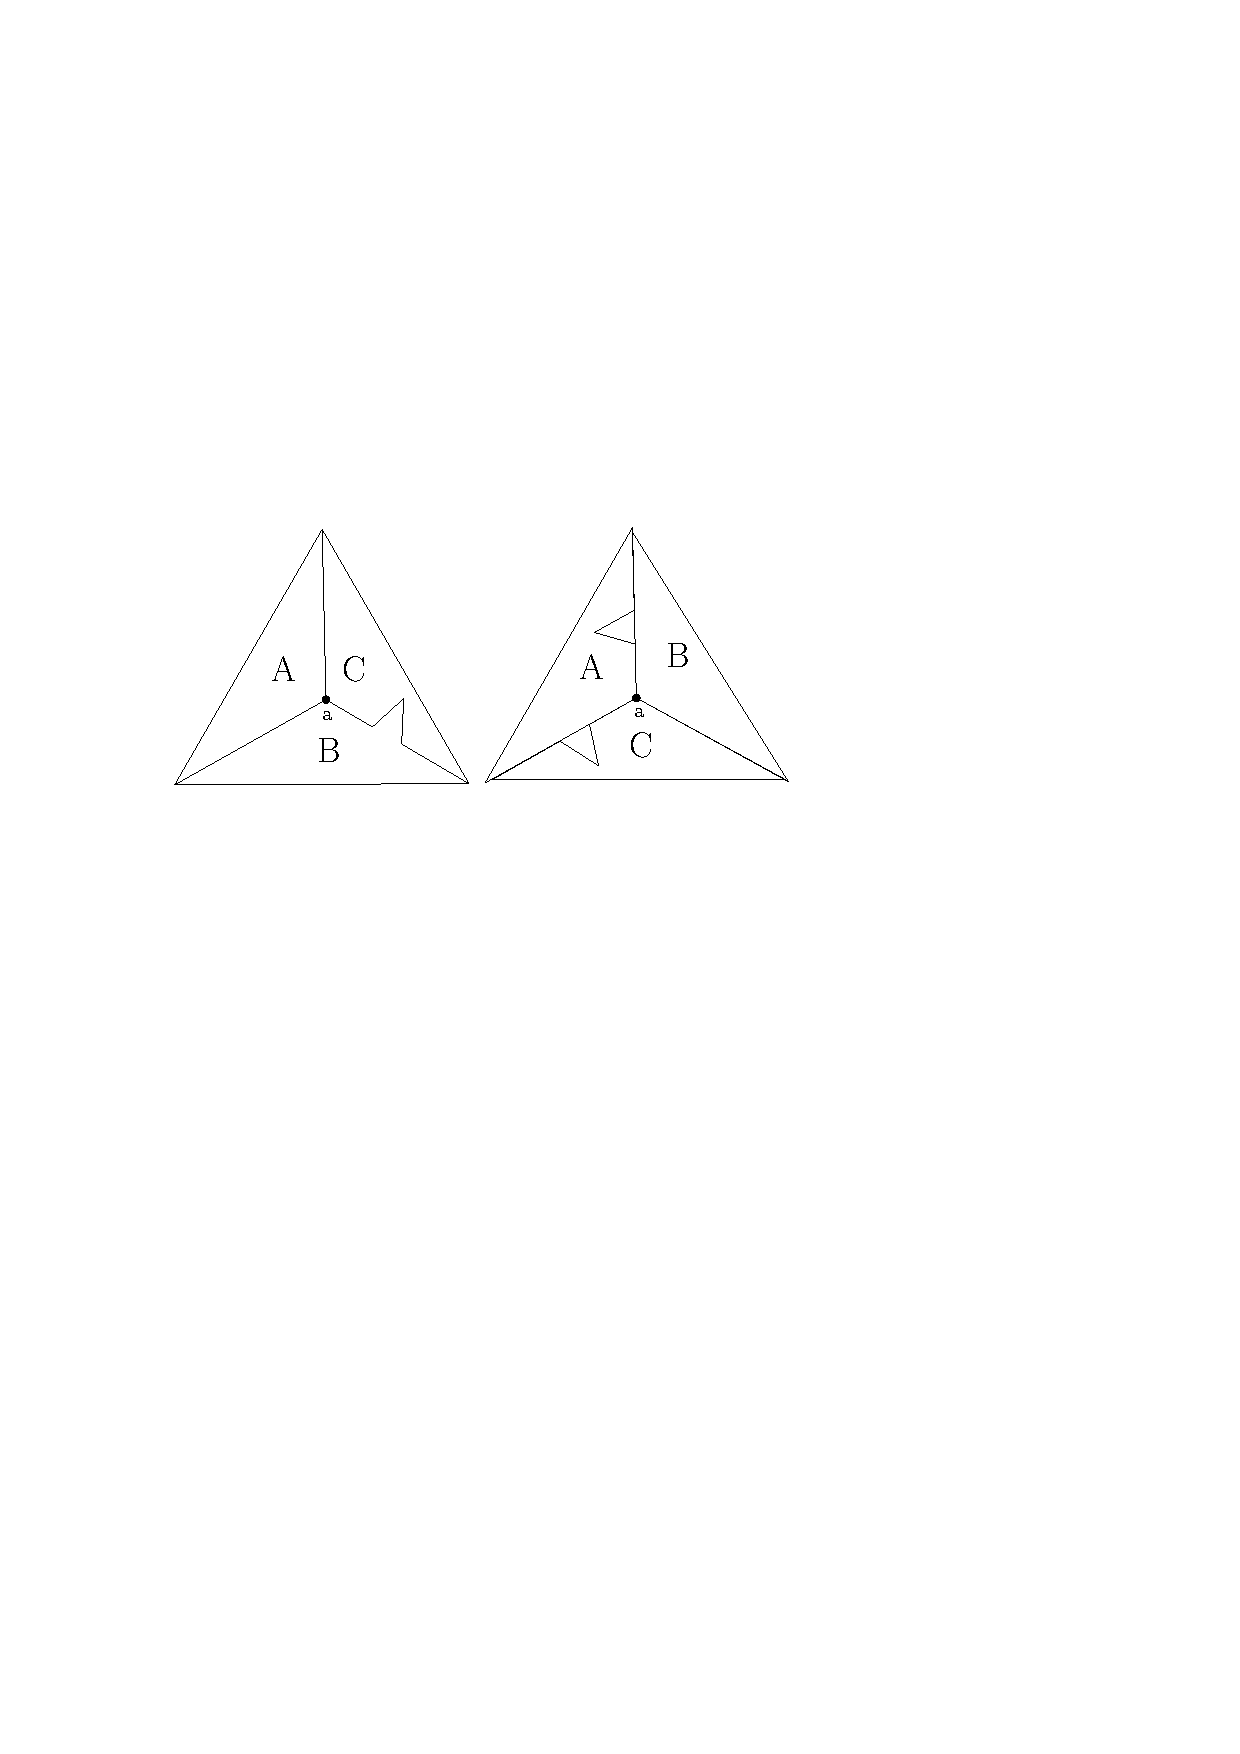
\includegraphics[scale=1]{graphics/orderedFaces.pdf}
\caption{Here we have two realizations of a polygonal linkage with two different clockwise orderings (C,B,A) and (B,C,A) respectively.  Note that the realization with ordering (B,C,A) has polygonal intersection.}
\end{center} 

\end{figure}

\newpage


\begin{thm}\label{thm:hinge2}
It is strongly NP-hard to decide whether a polygonal linkage whose hinge graph is a \textbf{tree} can be realized with fixed orientation.
\end{thm}

Our proof for Theorem \ref{thm:hinge2} is a reduction from {\sc Planar-3-SAT} (P3SAT): decide whether a given Boolean formula in 3-CNF with a planar associated graph is satisfiable. The \emph{graph associated} to a Boolean formula in 3-CNF is a bipartite graph where the two vertex classes correspond to the variables and to the clauses, respectively; there is an edge between a variable $x$ and a clause $C$ iff $x$ or $\neg x$ appears in $C$. See Fig.~\ref{fig:assoc} (left).


\begin{figure}[!htbp]
	\centering
	\includegraphics[width=0.7\columnwidth]{graphics/fig-assoc-hex.pdf}
	\caption[]{Left: the associated graph $A(\Phi)$ for a Boolean formula $\Phi$.
Right: the schematic layout of the variable, clause, and transmitter gadgets in our construction.}
	\label{fig:assoc}
\end{figure}





\subsection{Geometric Dissections}
The Wallace-Bolyai-Gerwien Theorem simply states that two polygons are congruent by dissection iff they have the same area.  A \textit{dissection} being a collection of smaller polygons that when hinged together form a polygon.  Here dissections don't have to be hinged.  Hinged dissections preserve adjacent polygon relationships and their points of connection.  The question of whether two polygons of equal area have a hinged dissection was an outstanding problem until 2007 \cite{abbott2012hinged}.

The Haberdasher problem was proposed in 1902 by Henry Dudeney which dissects an equilateral triangle into a square.
\begin{figure}[!htbp]
\begin{center}
\includegraphics{graphics/HaberdasherProblem.pdf}
\end{center}
\caption{The Haberdasher problem was proposed in 1902 and solved in 1903 by Henry Dudeny.  The dissection is for polygons that forms a square and equilateral traingle
 }
\label{fig:polygonallinkage-5}
\end{figure}
\newpage
\begin{figure}[!htbp]
\begin{center}
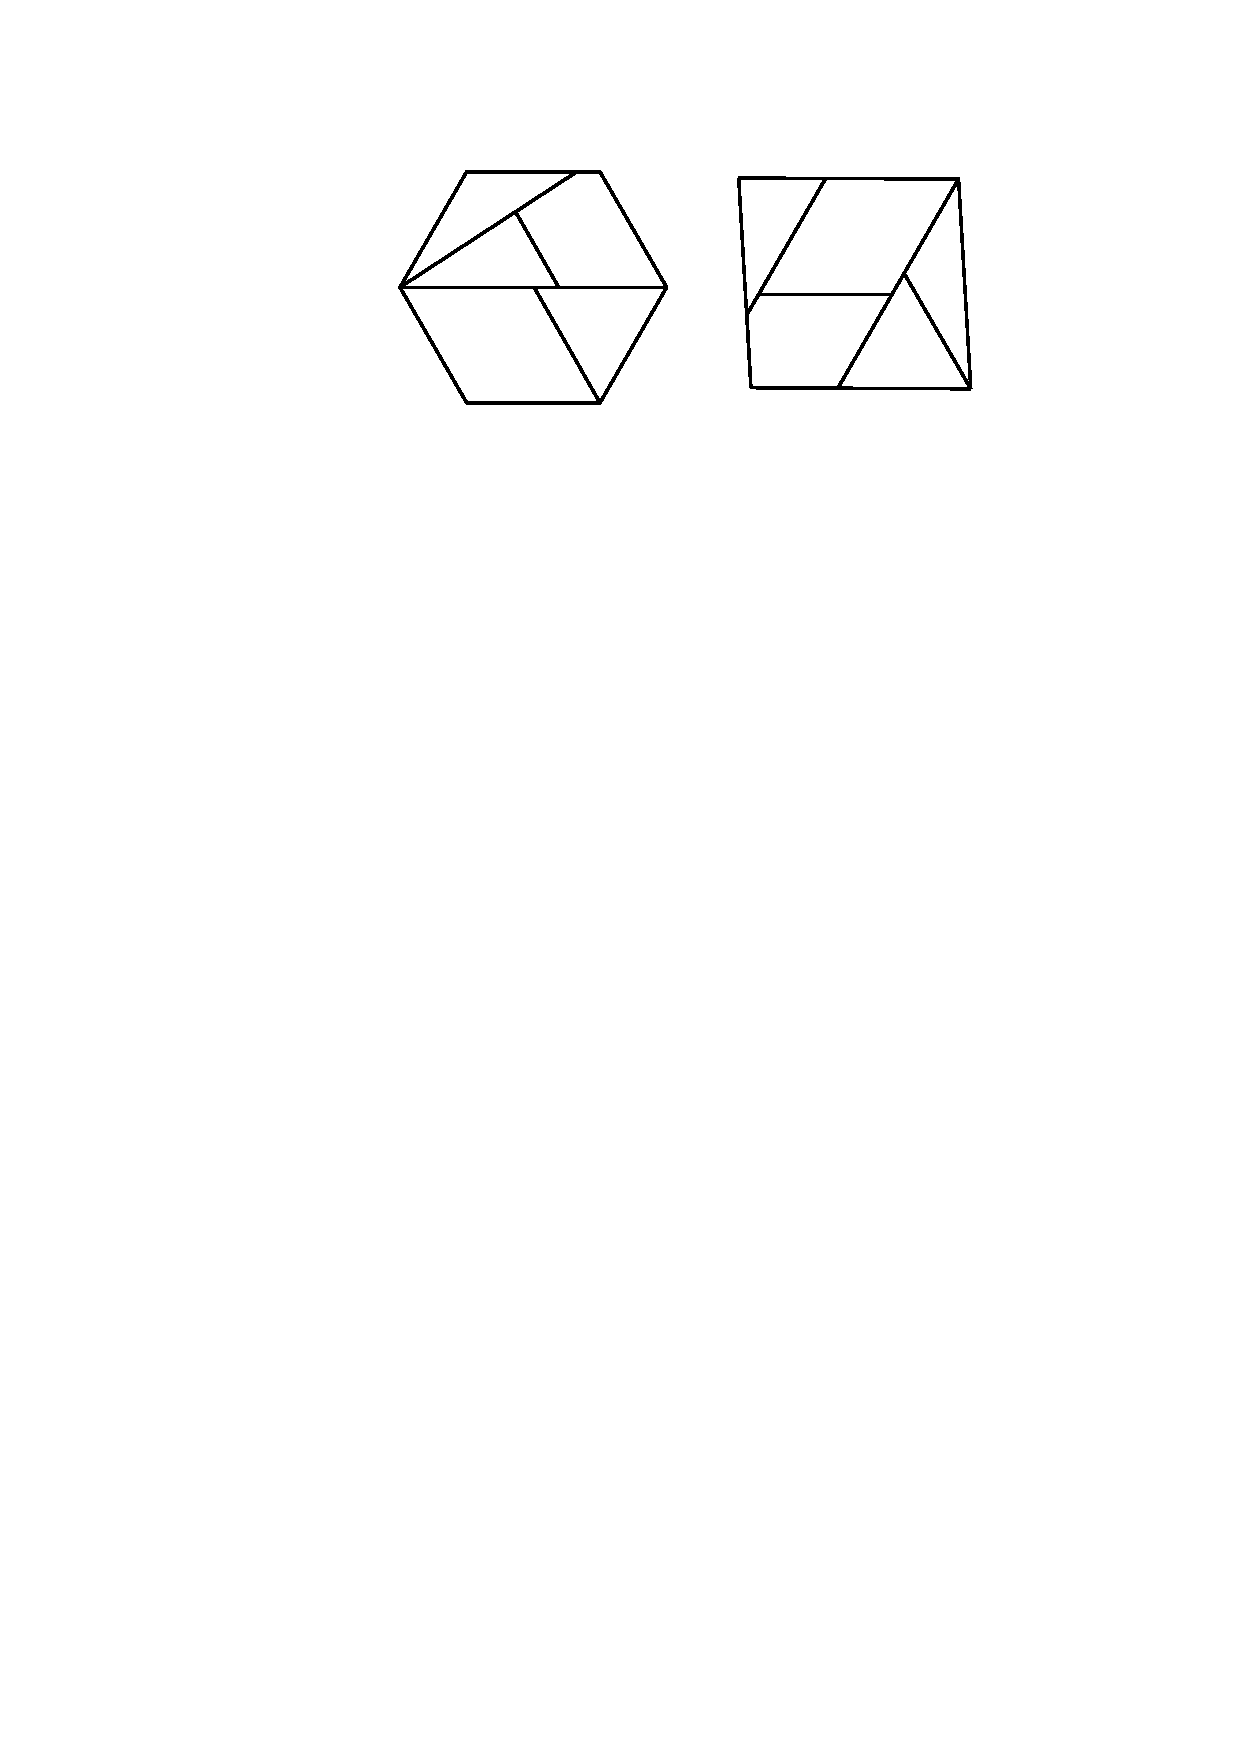
\includegraphics{graphics/GeometricDissectionBusschop.pdf}
\end{center}
\caption{Two configurations of polygonal linkage where the polygons touch on boundary segments 
instead of hinges.  These two realizations of the polygonal linkage are invalid to our definitions. 
 }
\label{fig:polygonallinkage-4}
\end{figure}
Geometric dissections are closely related to polygonal linkages.  Figure \ref{fig:polygonallinkage-4} shows two arrangements of the same polygons to form a hexagon and a square.  The reason these polygons are not polygonal linkages is that the polygons do not have consistent hinge points.  Figure \ref{fig:HingedTriangleSquare}, shows the Haberdasher problem with hinges.  This makes the Haberdasher problem as a type of polygonal linkage where the polygons are free to move about their hinge points and take the form of a triangle or square.
\begin{figure}[!htbp]
\begin{center}
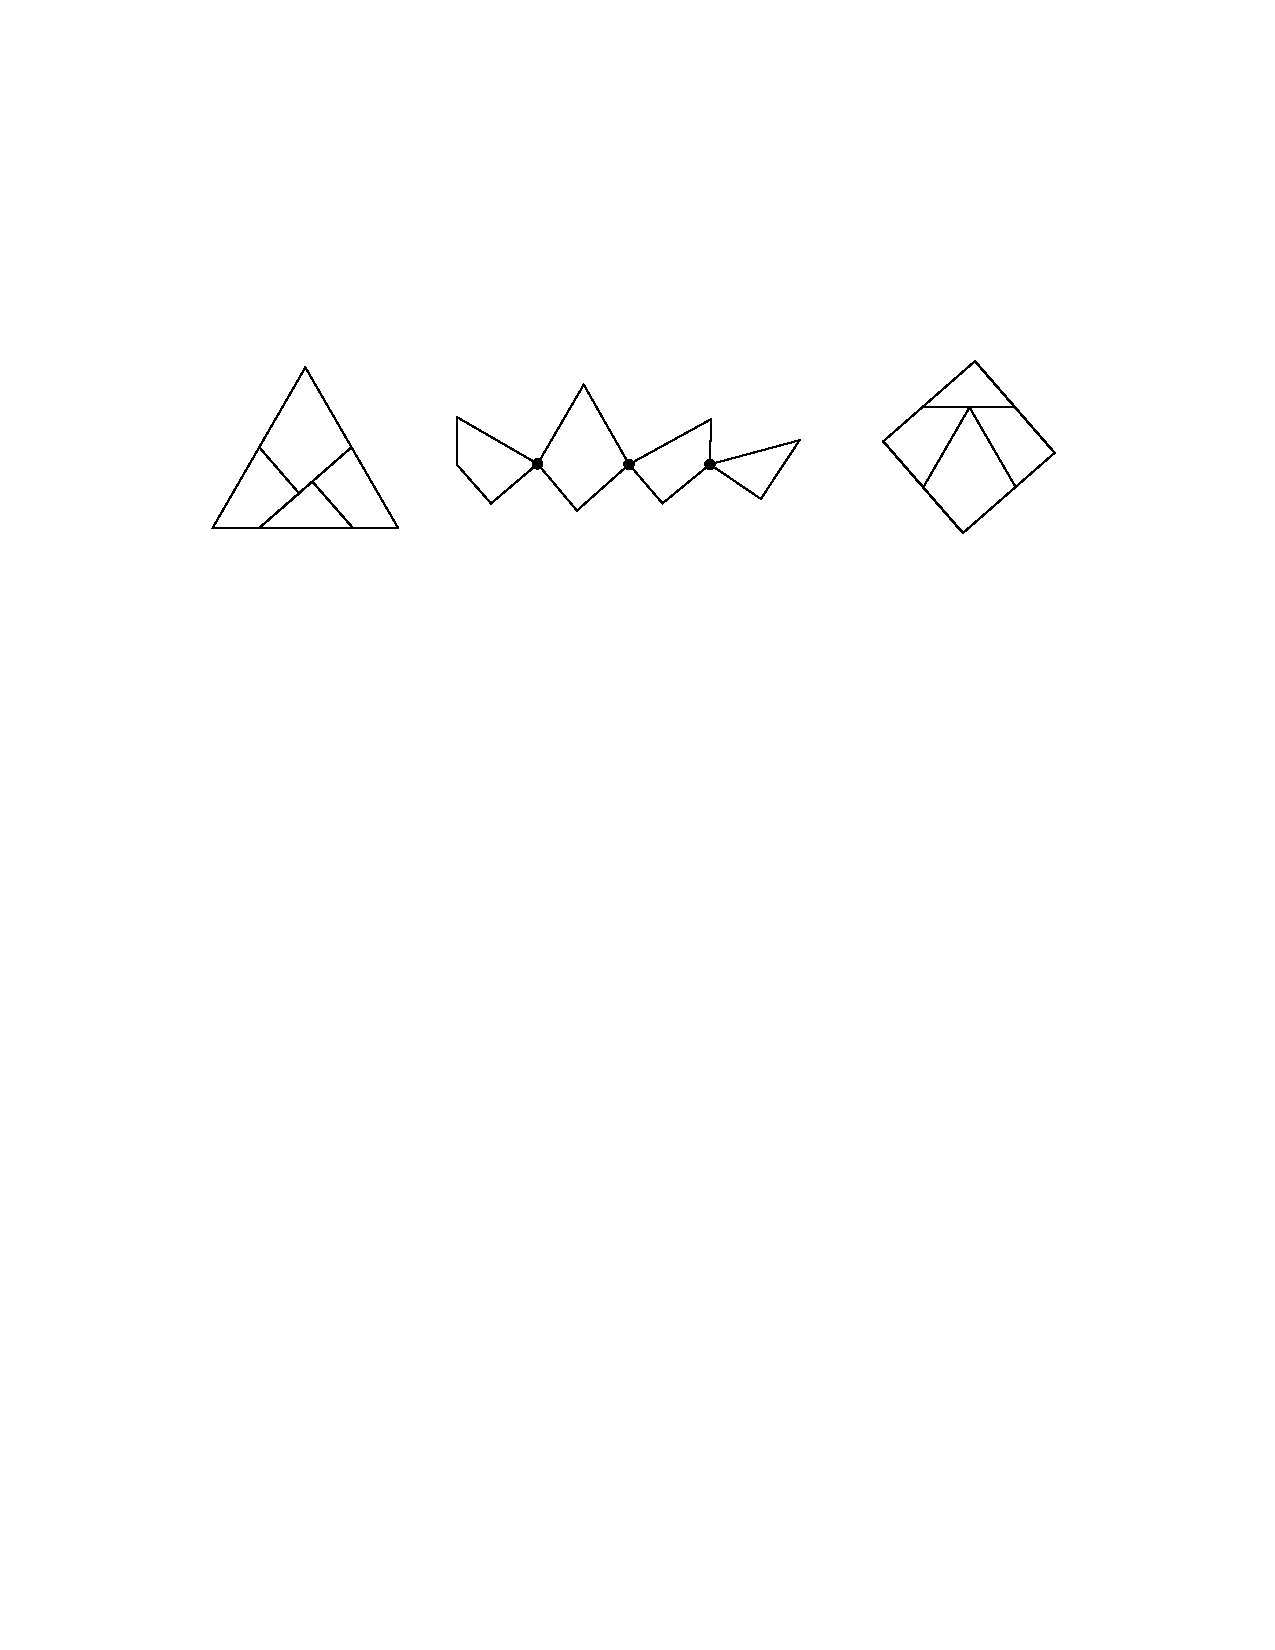
\includegraphics{graphics/HingedTriangleSquare.pdf}
\end{center}
\caption{This shows the Haberdasher problem in the form of polygonal linkage.}
\label{fig:HingedTriangleSquare}
\end{figure}




% With three cuts, dissect an equilateral triangle into a square. The problem was first proposed by Dudeney in 1902, and subsequently discussed in Dudeney (1958), and Gardner (1961, p. 34), Stewart (1987, p. 169), and Wells (1991, pp. 61-62). The solution can be hinged so that the four pieces collapse into either the triangle or the square. Two of the hinges bisect sides of the triangle, while the third hinge and the corner of the large piece on the base cut the base in the approximate ratio 0.982:2:1.018.



% %%%%%%%%%%%%%%%%%%%%%%%%%%%%%%%%%%%%%%%%%%%%%%%%%%%%%%%%%%%%%%%%%%%%
% %%%%%%%%%%%%%%%%%%%%%%%%%%%%%%%%%%%%%%%%%%%%%%%%%%%%%%%%%%%%%%%%%%%%
% %%%%%%%%%%%%%%%%%%%%%%%%%%%%%%%%%%%%%%%%%%%%%%%%%%%%%%%%%%%%%%%%%%%%
% %%%%%%%%%%%%%%%%%%%%%%%%%%%%%%%%%%%%%%%%%%%%%%%%%%%%%%%%%%%%%%%%%%%%
% %%%%%%%%%%%%%%%%%%%%%%%%%%%%%%%%%%%%%%%%%%%%%%%%%%%%%%%%%%%%%%%%%%%%
% %%%%%%%%%%%%%%%%%%%%%%%%%%%%%%%%%%%%%%%%%%%%%%%%%%%%%%%%%%%%%%%%%%%%
% %%%%%%%%%%%%%%%%%%%%%%%%%%%%%%%%%%%%%%%%%%%%%%%%%%%%%%%%%%%%%%%%%%%%
% \begin{figure}[h]
% \begin{center}
% 
\includegraphics[scale=1]{graphics/hingeOnThreeDistinctPolygons.pdf}
% \end{center} 
% \caption{(a) A polygonal linkage with a non-convex polygon and two hinge points corresponding to 
% three polygons.  Note that hinge points correspond to two distinct polygons.(b) Illustrating that 
% two hinge points can correspond to the same boundary point of a polygon.}
% \label{fig:linkage-1}
% \end{figure}
% %describe how it is a generalization of Linkages.
% A generalization of linkages are polygonal linkages where the edges of given lengths are replaced 
% by rigid polygons.  Formally, a \textit{polygonal linkage} is an ordered pair $\left(\PP,\HH 
% \right)$ where $\PP$ is a finite set of polygons and $\HH$ is a finite set of hinges; a 
% \textit{hinge} $h\in \HH$ 
% corresponds to two points on the boundary of two distinct polygons in $\PP$.  A \emph{realization} 
% of a polygonal linkage is an interior-disjoint placement of 
% congruent copies of the polygons in $\PP$ such that the points corresponding to each hinge are 
% identified (Fig. \ref{fig:1}). 
% A \textbf{realization with orientation} uses only translated or rotated copies of the polygons in $\PP$ (no reflections) and for each hinge, the cyclic order of incident polygons is given. 
% The topology of a polygonal linkage can be represented by the \textbf{hinge graph}, a bipartite graph where the vertices correspond to polygons in $\PP$ and the hinges in $H$, and edges represent the polygon-hinge incidences.
% This definition of realization rules well known geometric 
% dissections (e.g. Fig. \ref{fig:polygonallinkage-4}).
% %this is where the geometric dissection figure belongs
% \begin{figure}[h]
% \begin{center}
% 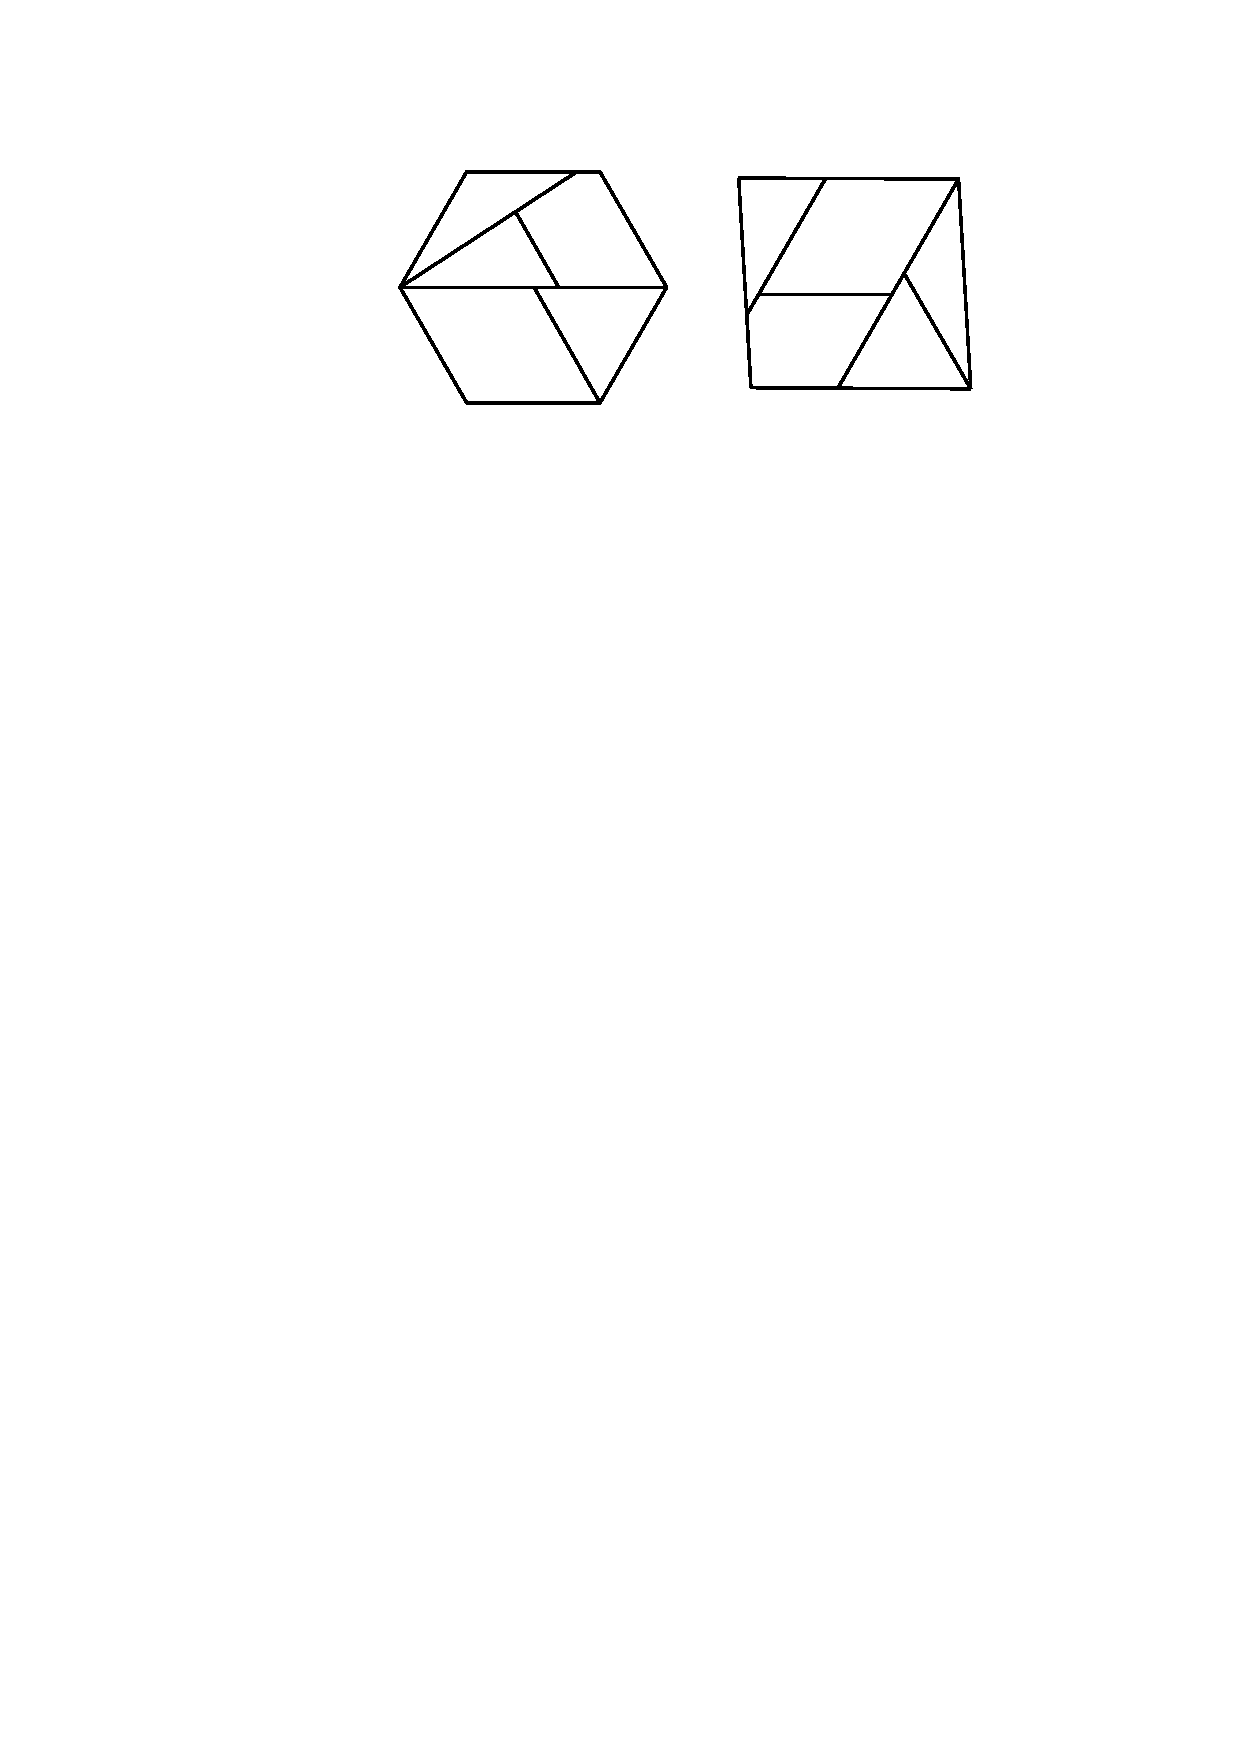
\includegraphics{graphics/GeometricDissectionBusschop.pdf}
% \end{center}
% \caption{Two configurations of polygonal linkage where the polygons touch on boundary segments 
% instead of hinges.  These two realizations of the polygonal linkage are invalid to our definitions. 
%  }
% \label{fig:polygonallinkage-4}
% \end{figure}

% \begin{figure}[h]
% \begin{center}
% 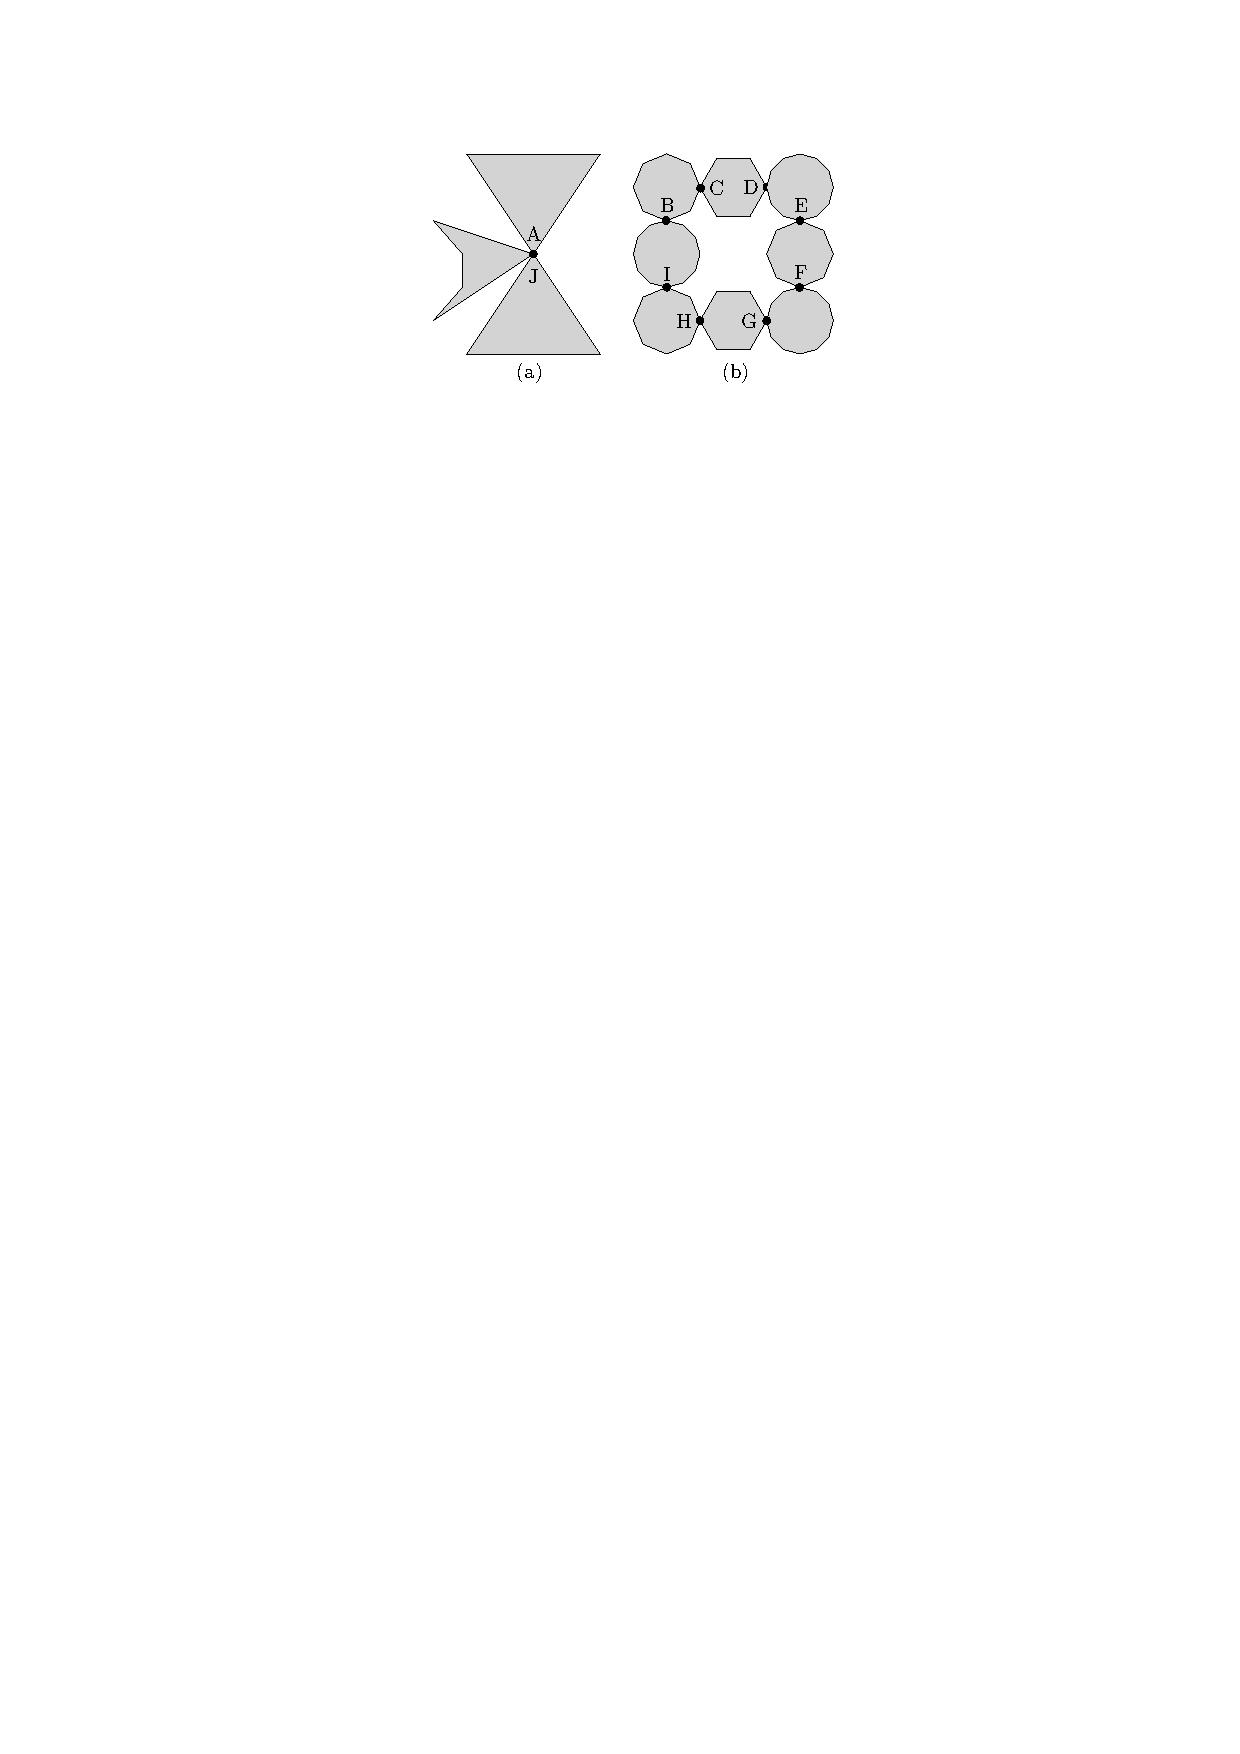
\includegraphics[scale=1]{graphics/linkageillustration.pdf}
% \end{center} 
% \caption{(a) A polygonal linkage with a non-convex polygon and a hinge point corresponding to three 
% polygons.  (b) A polygonal linkage with 8 regular polygons.}
% \label{fig:linkage-2}
% \end{figure}
% %%%%%%%%%%%%%%%%%%%%%%%%%%%%%%%%%%%%%%%%%%%%%%%%%%%%%%%%%%%%%%%%%%%%
% %%%%%%%%%%%%%%%%%%%%%%%%%%%%%%%%%%%%%%%%%%%%%%%%%%%%%%%%%%%%%%%%%%%%
% %%%%%%%%%%%%%%%%%%%%%%%%%%%%%%%%%%%%%%%%%%%%%%%%%%%%%%%%%%%%%%%%%%%%
% %%%%%%%%%%%%%%%%%%%%%%%%%%%%%%%%%%%%%%%%%%%%%%%%%%%%%%%%%%%%%%%%%%%%
% %%%%%%%%%%%%%%%%%%%%%%%%%%%%%%%%%%%%%%%%%%%%%%%%%%%%%%%%%%%%%%%%%%%%
% %%%%%%%%%%%%%%%%%%%%%%%%%%%%%%%%%%%%%%%%%%%%%%%%%%%%%%%%%%%%%%%%%%%%
% %%%%%%%%%%%%%%%%%%%%%%%%%%%%%%%%%%%%%%%%%%%%%%%%%%%%%%%%%%%%%%%%%%%%

% For the remainder of this thesis, we'll focus on the polygonal linkages with the following 
% restrictions:
% \begin{enumerate}
% \item Embedded polygons must be convex, i.e. for any two embedded points $u,v \in P'$, the set:
% $$\left\lbrace u  \cdot t + (1-t) \cdot v : t \in [0,1] \right\rbrace \in P'$$
%  \item  Polygons can only intersect at hinge points.  No two polygons can intersect at 
% their boundary or interior with the exception of possible a hinge point.  
% \end{enumerate}